%!TEX root = ../report.tex

%
% Architecture
%

\section{Architecture} % (fold)
\label{sec:architecture}

This work will follow the architecture described in Figure~\ref{fig:architecture}.
There will be a module in Racket that will provide a Racket interface for the rest of the system using \emph{Racket FFI}. Is through this interface that the users will interact with the system. This will be a layer that will not have an impact on performance.


\begin{wrapfigure}{r}{0.5\textwidth}
	\vspace{-15pt}
    \centering
	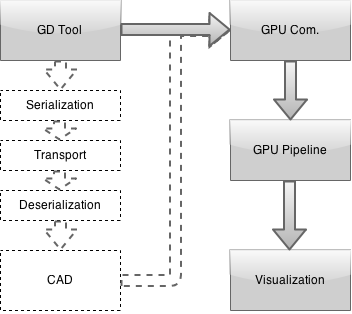
\includegraphics[width=0.5\textwidth]{img/Architecture/GD-Fast-Pipeline.png}
	\caption{High Level Architecture}
	\label{fig:architecture}
	\vspace{-15pt}
\end{wrapfigure}

The second step is the OpenGL layer, that implements the Racket interface and then creates the window and manages user input. The functions provided to Racket will create here the description of the geometry that will be \emph{amplified} in the next phase. This description is one $GL\_POINT$ that represent each geometric primitive and is embedded with an array of floats that encode the position, the type of geometry and specific information like size or number of sides. 

In the last step are the shaders, where most of the work is done. This receives the small description of the geometry and generates the primitives to be drawn. To achieve this, it is applied the concept of geometry amplification. As explained in Section~\ref{sub:geometriy_shaders}, this method has limitations that could make an impact on how the geometry generation is implemented. However OpenGL guarantees support for at least 256 vertices which is enough to generate the majority of geometric primitives. Since this problem is hardware dependent and GPU hardware is getting more powerful this should not be a problem in the near future. 
To achieve high performance with this system, will be explored and implemented within this module the concepts of level of detail (LOD) and object culling. The first is related with the detail which each object is generated in relation with the camera position, generating  objects with high detail when they are close to the camera and to progressively lose detail when move away from the camera.  At the same time, objects that are partly or completely covered by other are generated in order to decrease the detail or even prevent them from being generated.

This architecture significantly reduces the amount of data that is moved between layers and takes advantage of the power that recent GPUs have.

For instance the following code results in the Figure~\ref{fig:pic1} that is a procedural generated model of a city with ~40k buildings. This example was generated with the current prototype with the following Racket code:


%\begin{lstlisting}[frame=single,language=Lisp]

\lstset{style=racket}
\begin{lstlisting}
(define (building x y z w l h)
  (let ([h1 (* 0.7 h)]
        [h2 (* 0.4 h)])
    (begin
      (box x y h1 w l h1)
      (cylinder x y (+ (* h1 2) h2) (* 0.7 w) h2))))

(init 1000)

(let ([grid-size 30.0])
  (for* ([xi  (in-range (- grid-size) grid-size 0.3)]
         [yi  (in-range (- grid-size) grid-size 0.3)])
    (building xi yi 0.0 0.1 0.1 (random))))

(start)
\end{lstlisting}
%\begin{absolutelynopagebreak}

%\end{absolutelynopagebreak}

The \emph{init} command makes an initialization of the system and its argument is an estimation of the number of primitives just for optimization purposes, the \emph{start} command creates the window and starts the visualization. In between the model is created, in this case the code that creates a squared city model with buildings of random hight.

\colocarFiguraMaisRodada

\begin{figure}[htb]
	\centering
	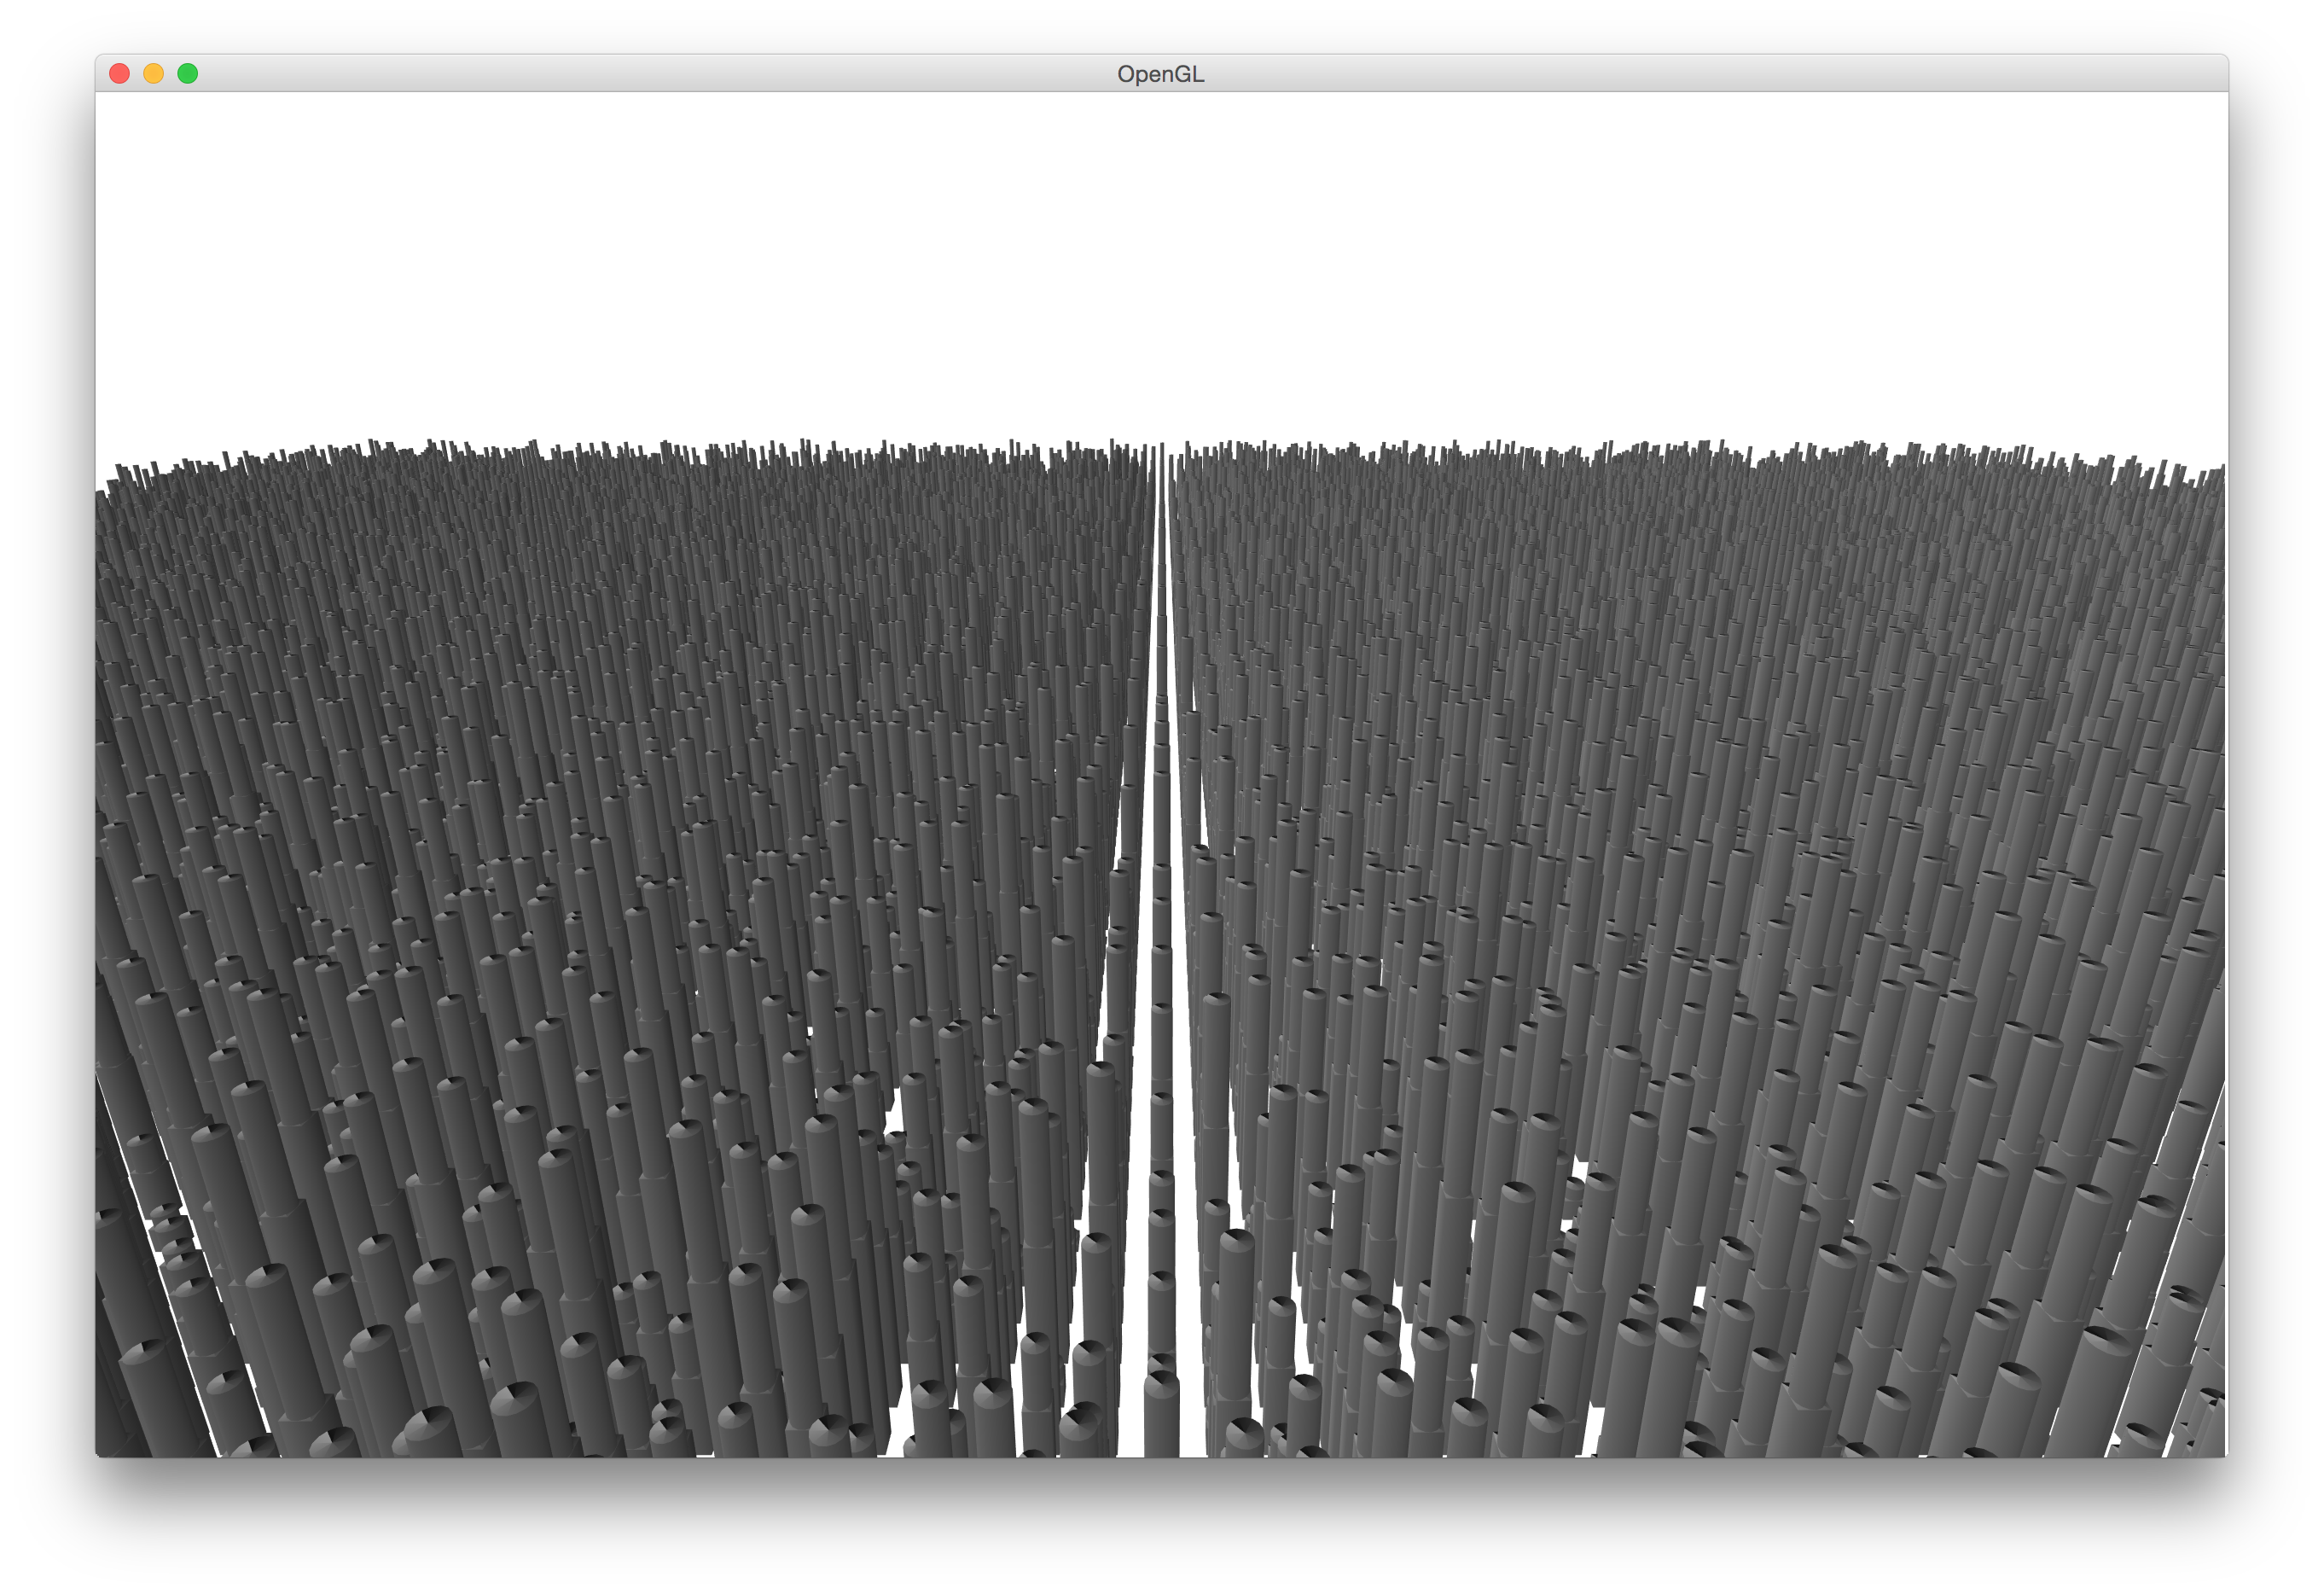
\includegraphics[width=0.95\textwidth]{img/Solution/City4-racket.png}
	\caption{City with ~40k buildings}
	\label{fig:pic1}
\end{figure}



% section architecture (end)
